\subsection{Geschichte}\label{geschichte}

Design-Fehler, inkorrekte Installationen und Mutwillige Angriffe zählen mit zu den Risiken in Software-Systemen. Sie können beispielsweise zu falschen oder zu spät eintreffenden Ergebnissen, Datenverlusten und als weitere Folge zu wirtschaftlichen und persönlichen Schäden führen \cite{Laprie:1995:DCC:1899254.1899261}.
Eine typische Herangehensweise der Softwareentwicklung um Fehler in Programmen zu vermeiden, besteht in der möglichst vollständigen Eliminierung von Design-Fehlern vor der Ausführung im produktiven Betrieb \cite{Avizienis:1975:FFC:800027.808469}. 
Die Idee, durch redundante Berechnungen von Ergebnissen Fehler zu erkennen und zu vermeiden, geht lange zurück. Bereits 1834 schrieb der irische Naturwissenschaftler Dionysius Lardner: \enquote{\emph{The most certain and effectual check upon errors which arise in the process of computation,	is to cause the same computations to be made by separate and independent computers; and this	check is rendered still more decisive if they make their computations by different methods.}} \cite{lardner}.

Mit der Motivation, vor allem Laufzeitfehler, die aufgrund von Design-Fehlern auftreten, zu vermeiden, erschienen Anfang der 1970er Jahre Vorschläge zum Einsatz von mehreren funktional äquivalenten Versionen des Zielprogramms \cite{methodology}.
Eine Auslegung des Konzepts der Verwendung von Redundanz zum Erzielen von fehlertoleranten Systemen wurde bereits 1974 als \enquote{Recovery Block}-Ansatz bekannt \cite{Horning:1974:PSE:647641.733522}.
Hierbei werden Ergebnisse eines primären Blocks des Programms, wie in Abbildung \ref{graph-recovery} angedeutet, durch einen Akzeptanztest überprüft.
Falls der Akzeptanztest bei dem primären Block scheitert,wird der erste sekundäre Block ausgeführt. Dieser Prozess wird wiederholt bis ein Akzeptanztest das Ergebnis eines Blocks akzeptiert oder das System aufgrund mangelnder weiterer Blocks abbricht.
%
%
\begin{figure}[ht]
	\centering
	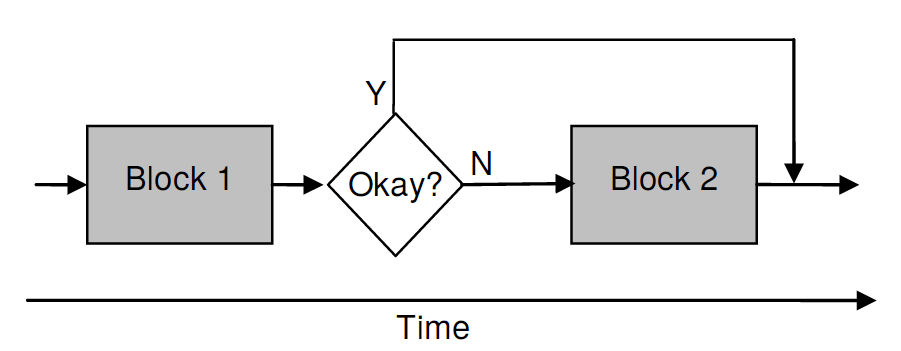
\includegraphics[width=0.8\textwidth,natwidth=901,natheight=333]{grafiken/recovery-block.png}
	\caption{Prinzip der Recovery-Blocks \cite{lardner}}
	\label{graph-recovery}
\end{figure}
%
%
Der zunächst als \enquote{redundant programming} bezeichnete Ansatz, einen systematischen Prozess zur Entwicklung von funktional equivalenten, multiversionalen Programmen, zu definieren, wurde später in \enquote{N-version programming} umbennant.
Wie in Abbildung \ref{graph-n-version-single} ersichtlich, liegt der wesentliche Unterschied zum Ansatz der Recovery-Blocks darin, dass die als Versionen bezeichneten Blöcke in jedem Fall alle ausgeführt werden und statt eines Akzeptanztests ein Voting auf Basis aller Ergebnisse der verschiedenen Versionen durchgeführt wird.
Die begründende Arbeit dazu veröffentlichten Liming Chen und Algirdas Avizienis 1977 mit \enquote{\emph{N-version programming: A fault-tolerance approach to reliability of software operation}} \cite{Chen1978}.
%
%
\begin{figure}[ht]
	\centering
	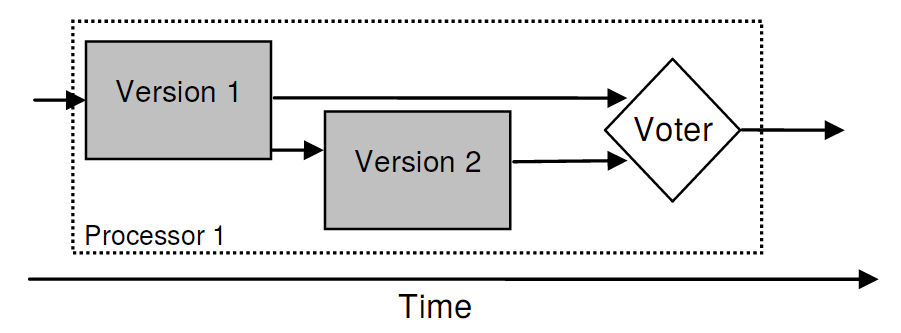
\includegraphics[width=0.8\textwidth,natwidth=901,natheight=333]{grafiken/single-thread-n-version.png}
	\caption{Voting Prinzip in der N-Version Programmierung bei Single threading \cite{lardner}}
	\label{graph-n-version-single}
\end{figure}
%
%

\subsection{Konzepte} \label{konzepte}

- Definition
- assumptions in the reasoning for this approach
- Process of building software
- used concepts
- mechanisms
- critical points

